\documentclass{article}
\usepackage{graphicx}
\usepackage[utf8]{inputenc}
\usepackage[margin= 3.5cm, includefoot]{geometry}
\usepackage{caption}
\usepackage{subcaption}
\usepackage{amsmath}
\usepackage{mathtools}
\usepackage{float}
\usepackage{verbatim}
\usepackage{ulem}

\title{Mind Your Hinglish}
\author{\hspace{0.55cm}Aniket Gupta\hspace{2cm}Aayush Goyal\hspace{2cm}Anshuman Panda\\2019CS10327\hspace{2.2cm}2019CS10452\hspace{2.4cm}2019CS10463}

\date{October-November 2021}

\begin{document}

\maketitle

\section{Introduction}
Were you taught Hindi in your school? What about English? Have you ever thought ki inn dono mein se zyada frequently tum konsi language use krte ho? And did you just realize that the former line contains morphemes of both Hindi and English? Do you know this mixing of Hindi and English has got \sout{official} name called Hinglish? Most of the academic curicullums frown upon mixing of Hindi and English, so here we will be discussing more on the depths and breadths of Hinglish.
\\\\
Hinglish, the language used by most of the Indian natives nowadays is a blend of both Hindi and English. It is a macaronic use of English with Hindi morphemes involving code switching and code mixing between these languages where they are freely interchanged according to the ease of use. This is widely in use because of the ease of speaking and writing. Mostly the people are not very frequent in using English and nor are they very proficient in pure Hindi and hence are observed to use a mix of these both, that is, Hinglish. Such code mixing and code switching has crept it's way into advertisements, newspapers, magazines, TV shows, Bollywood movies as well as the corridors of political and corporate powers in India. 
% TODO: write some survey about the ease of use between these thre laanguages. 
\\\\
Have you ever thought about how did Hinglish came to be? Have you ever thought how it became the language of the common even if it is not taught in any school and curicullum? Even the poeple who have not received any formal education in any of these 2 languages are seen using it in their daily life. How long do you think Hinglish has been in existence? Is it limited to the modern Indian youth influenced by the social media platforms? or it has been in existence much before the social media platforms became popular? What all do you think has given rise to the rapid growth in popularity of hinglish? Is it limited to the "upper-class elite" Indians or is it used in the semi-urban and the rural centres as well? 

\section{Rise of Hinglish}
It is a general misconception that this language has came into existence because of the influence of modern social media platforms and internet on the modern Indian elite class groups. In fact the use of hinglish can be traced back to time when India was under british rule. The British government at that time used english but most of the Indian were not good in English. These interaction of English and Hindi speakers led to the use of words of both the languages to some extent by both sides, the government and the people. An example of use of hinglish by the educated class, during the british rule can be observed in the words of Ayodhya Prasad Khatri (1857-1905), a prominent hindi poet. He wrote:
\begin{quote}
    \centering
    \textit{Rent Law ka gham karen ya Bill of Income Tax ka?\\
    Kya karen apan nahiin hai sense right now-a-days.\\
    Darkness chhaaya hua hai Hind men chaaro taraf\\
    Naam ki bhi hai nahiin baaqi na light now-a-days.}
\end{quote} 
The ease with which the poet has criticised the British Government tax laws by mixing and switching between words of Hindi and English language clearly shows the prevalence of Hinglish at that time. There are few other written proofs that support the use of Hinglish during \textbf{"British-Raj"}. Even the word "British-Raj" is itself a Hinglish word. \\
Although these examples support the fact that Hinglish has been in use since long back, it didn't gain much popularity until much later. Author Shobha De, also known as the "Jackie Collins of India", used Hinglish in her writings in the 1960s. In the late 1990s, the arrival of many television channels like MTV and Channel V, advertisements by many companies using both Hindi and English vocabulary, development of entertainment industry really exploded the combined use of Hindi and English. Television channels and radio stations in the country freely moved between the two languages. The phrase \textit{"Chitrahaar ke prayojak hain..."} was slowly replaced by \textit{"milte hain brea ke baad}". \\
Slowly, growing popularity of social media platforms among the Indian youth during the beginning of 21st century further boosted the growth in the popularity of Hinglish. In 2005, author B.K. Mahal wrote \textit{"The Queen's Hinglish: How to Speak Pukka Dictionary"}. It contains intriguing facts and stories and illustrated throughout how Hinglish is becoming an international phenomenon due to the internet and the growth of Bollywood film industry in India. In 2011, to increase cooperation in official activities, Official Language Department of Indian Home Affairs Ministry issued a Circular to promote the use of Hinglish instead of pure Hindi language term to ease the working of officials, according to new techniques. In same year, Rita Kothari and Rupert Snell published \textit{"Chutnefing English: The phenomenon of Hinglish"}. All these references show that how Hinglish has developed over the years.

\section{Advertisements, TV shows, Newspaper, Entertainment}
The rise of Indian media in the late 90s gave a major boost to the spread of Hinglish. Many of the multinational companies were trying to increase there reach among the general public in India. Many of these companies, that earlier advertised in English, were now shifting to use both Hindi and English language in there advertisements. The first major company that used Hinglish in its advertisement was the American soft drink maker Pepsi.
\begin{quote}
    \centering
    \textit{Yehi hai right choice, baby}\\
\textit{Yeh dil maange more}
\end{quote}

\begin{figure}[H]
\centering
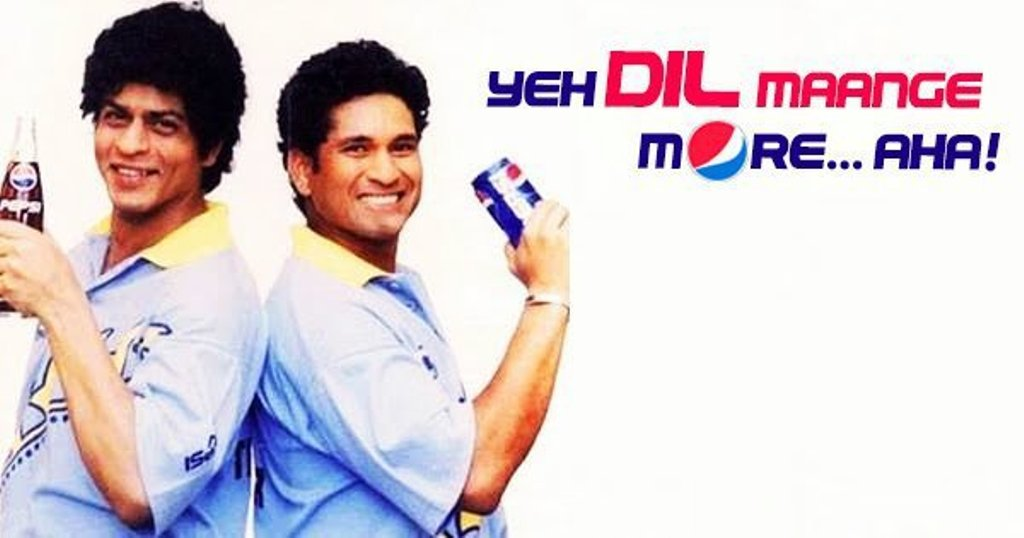
\includegraphics[width=0.5\textwidth]{images/pepsi.jpg}
\end{figure}

These Pepsi punchline slogans became so popular that the later became the battle cry of Indian Army during 1999 Kargil war. Mixing Hindi and English came very easily to the informal world of advertising. After Pepsi many other companies followed the same line and used jingles in Hinglish to advertise there products. FCB Ulka promoted milk by following popular jingle:
\begin{quote}
    \centering
    \textit{Piyo glass full doodh, dhoodh hai wonderful ... Pee sakte hai roj glass full\\
    Garmi me dalo doodh me ice ... Doodh bangaya very nice}

\end{quote}
Another such jingle is by the telecom service provider Airtel:
\begin{quote}
\centering
\textit{Chai ke liye jaise toashota hai ... Vaise har ek friend zaroori hota hai}. 
\end{quote}
Though these jingles do not appear to have any deep meaning in the advertisement they are nevertheless catchy and appears to influence and persuade the audience by use of funny code mixing patterns. Some other popular Hinglish taglines used in advertisements are shown below:
\begin{table}[H]
\centering
\begin{tabular}{|c|c|c|}
\hline
\textbf{Company} & \textbf{Taglines}\\
\hline \hline
Bajaj Coolers  & Ekdum solid cooling \\\hline
Dove & Naya Dove whitening deodorant \\\hline
Sprite & Bujhaye pyaas, baki all bakwas! \\\hline
Crest & Look Ma, no cavities! \\\hline
Domino’s pizza & Yeh hain rishton ka time \\\hline
Lays & Pal banaye magical \\\hline
Maggi Noodles & Taste bhi, Health bhi \\\hline
\end{tabular}  
\end{table} 
These punchlines have become so poular that many young people can be seen using these in day-to-day coversation.\\
The growth of Bollywood and Indian media has further popularised the use of Hinglish. A very popular song from which code-mixing and switching can be witnessed is 
\begin{quote}
    \centering
    \textit{Heer toh badi sad ... Aajkal very mad ... Heer toh badi sad \\
    Aajkal very mad ... Na khaati peethi ... Rona toh na mushkil}
\end{quote}
composed by A.R. Rahman and sung by Mika Singh and Nakash Aziz. Some popular Bollywood movies that have there tile in Hinglish are \textit{Kill Dil, Ek Villain, Super Nani, Jab We Met, Tanu Weds Manu}. Many of the news-shows and debates on news channels can be seen switching easily between Hindi and English. As clear from the above discussion, Hinglish has spread its tentacles in Advertisements, TV shows and Media. Over the years, it has become common household languages in small towns and villages as well.

\section {Social Media in Modern India}
Online platforms in recent times are one of the best examples of the usage of Hinglish in Modern India. The prevalence of digital communications in India has given rise to textspeak – a way of using abbreviations, slang and emoticons when writing online and in text messages. Hinglish has found its way to dominate conversations online. This is primarily because many people in India are bilingual, comfortable in speaking both English and Hindi, but prefer typing in English. Adding to this is the ubiquity of keyboards in the English alphabet, and in stark contrast, the virtual absence of Hindi keyboards. This has led to most people express their opinions and feelings in Hinglish. 

Many people in India have a Hindi as their mother tongue, and English has been largely used in formal occasions and official communications. Hindi has been the language (in most North Indian families) with which people conveyed emotions to their friends and family. Social media platforms have largely been used for connecting people, for expressing opinions, and maintaining relations. Naturally, there must be a personal touch to the conversations. When they communicate with family or friends on social media, or 'textspeak' with them, they tend to type in some Hindi words as well, attempting (and achieving) a sense of belonging. Hinglish has developed and grown popular in Twitter, WhatsApp, Facebook, Instagram and many other online platforms.

Indian Social Media influencers have also been taking on this trend, and examples can be found in Youtubers' videos, Instagram influencers' posts, Twitter posts, etc. Here is an example of an Instagram post, joking on the the 'importance' of 10th/12th marks:

\begin{figure}[H]
\centering

\includegraphics[width=0.45\textwidth]{images/meme.png}
\end{figure}

In the same way Hinglish developed, mixes of English and other Indian languages, like Odiya, Telugu, Marathi have also started becoming popular, and as social media have started to become an ubiquitous part of our lives, these mixes of languages only seem to become more and more famous, and be a part of our lives.


\section{Usage and Popularity among the people}
Given the increasing use of Hinglish in the modern world, we have gathered some results of the surveys on how indians prefer HInglish over Hindi and English. In this we have analysed the usage and popularity of Hinglish among the people from different age groups, regions and class of people. The survey conisited of 744 people and we have made 4 different categories to which the people belong to. The categories are as follows:
\begin{enumerate}
    \item \textbf{Age Group:} The age group to which they belong to.
    \item \textbf{Origin Factors:} The region to which they belong to.
    \item \textbf{Mother Tongue:} The mother tongue to which they belong to.
    \item \textbf{Frequent Usage:} The frequency of use of which Language by the people.
\end{enumerate}
And further in all of these groups we have focused on 4 aspects of usage and popularity of Hinglish. The 4 aspects are as follows:

\begin{enumerate}
    \item \textbf{Mixing of Languages:} How often use Hindi and English by mxing them, ie, as Hinglish.
    \item \textbf{Speed of Reading:} How fast the people read the Hinglish written in the Latin script (basically using words from English) rather than in the Devnagari script.
\end{enumerate}
Below is the analysis of different aspects of Hinglish for each group as stated above.

\subsection{Age Group}
The age groups can be broadly into the following categories:
\begin{enumerate}
    \item \textbf{Gen X:} People who are 44 and older. This is about 36.2\% of the respondents of survey.
    \item \textbf{Gen Y:} People who are 25 to 44. This is about 44.2\% of the respondents of survey.
    \item \textbf{Gen Z:} People who are 15 to 24. This is about 19.6\% of the respondents of survey.
\end{enumerate}
A detailed distribution of people belonging to different age groups is in the figure below:
\begin{figure}[H]
    \centering
    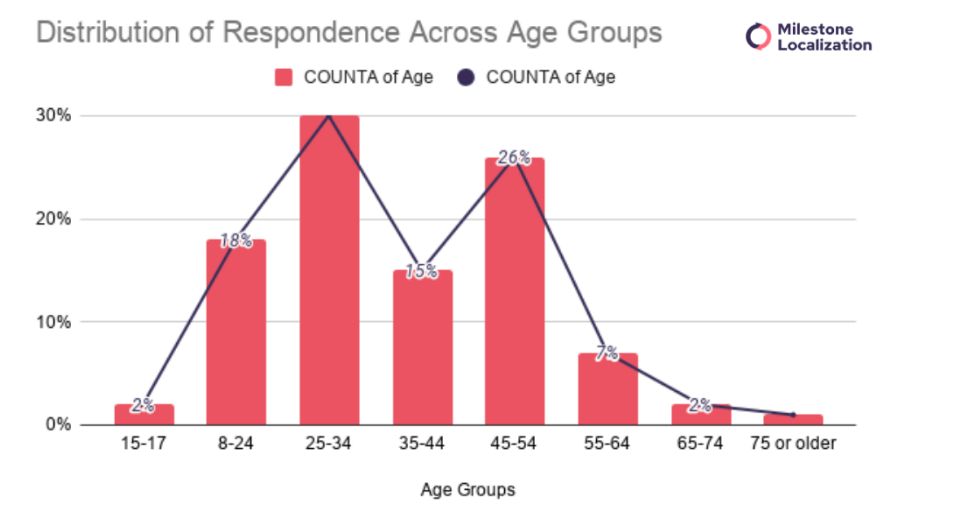
\includegraphics[width=0.8\textwidth]{plots/distribution_with_age.png}
\end{figure}

Now we will look at the usage and popularity of Hinglish among the people belonging to different age groups according to different aspects as stated above.

\subsubsection{Mixing of Languages}

\begin{figure}[H]
    \centering
    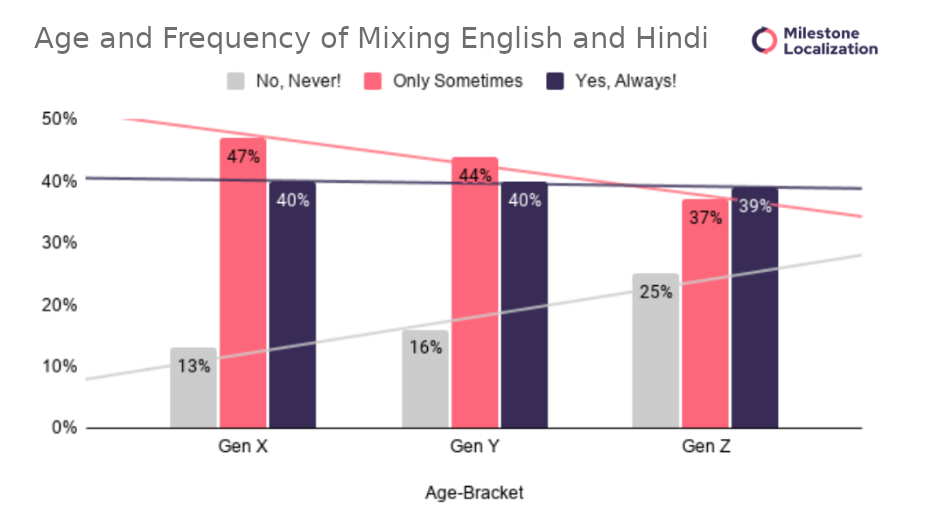
\includegraphics[width=0.8\textwidth]{plots/age_mixing_language.png}
\end{figure}
From the above it can be inferred that the people who are in the age group Gen X are more likely to use Hinglish than the people in the age group Gen Y and Z. As we would have normally expected that teh Gen Z, the current generation, who are getting more influenced by the social media platforms, are mixing the languages less than the other age groups. 

\subsubsection{Speed of Reading}

\begin{figure}[H]
    \centering
    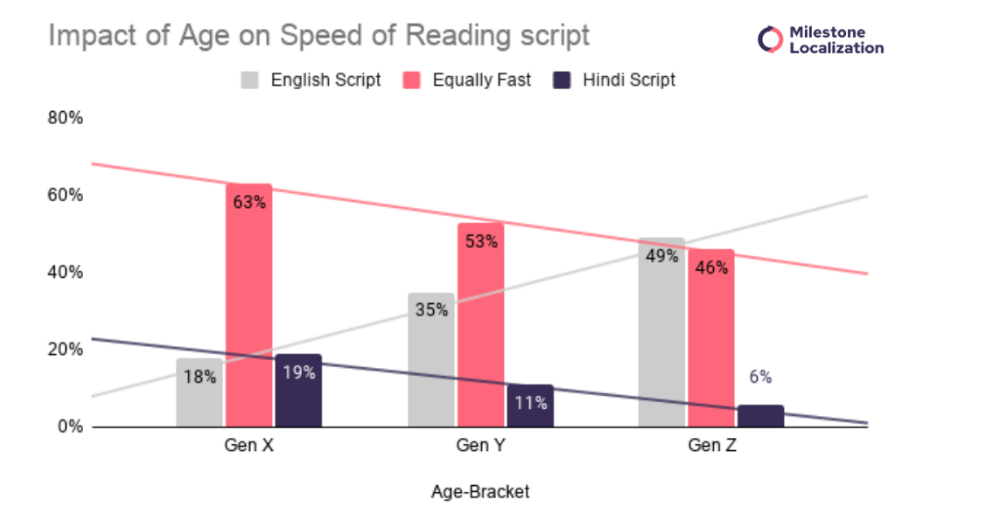
\includegraphics[width=0.8\textwidth]{plots/age_faster_read.png}
\end{figure}

From the above plot we can see that the people who are in the age group Gen Z are very less acquainted with the Hindi script. They mostly prefer to read it through the Latin script. They are more familiar wiht the English script one of the reasons being that most or the edication is nowadays done in the English language. Whereas in the older generation, as the education was in both Hindi and English, they are able to readd both of them equally fast.

\subsection{Origin Factors}

The people here have been divided based on the cities they belong to. The cities have been classified into 'big' metro cities like Delhi, Mumbai, etc and then the Tier 1 cities like Jaipur, Ahmedabad, etc. The rest of the cities have been classified into Tier 2 and Tier 3, the cities like Ajmer and Ludhiana. Below is the graph of distribution of people belonging to different cities:

\begin{figure}[H]
    \centering
    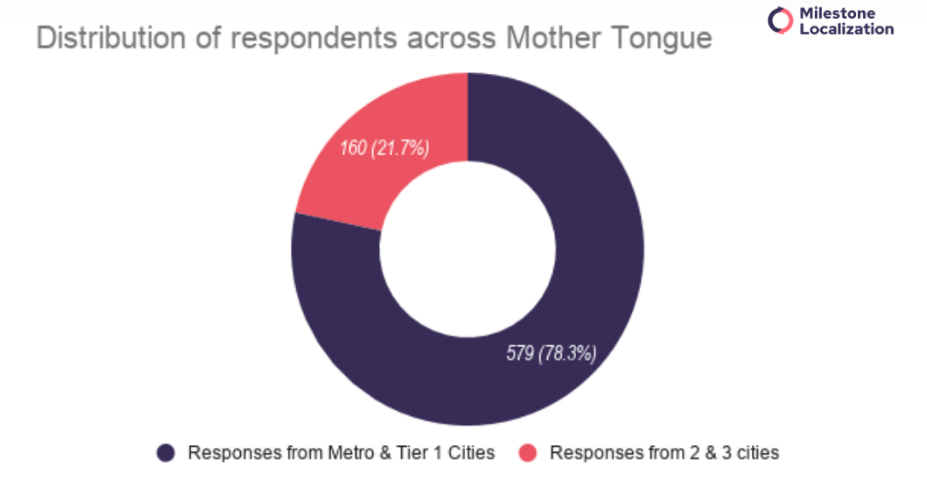
\includegraphics[width=0.8\textwidth]{plots/distribution_with_city.png}
\end{figure}

\subsubsection{Mixing of Languages}

\begin{figure}[H]
    \centering
    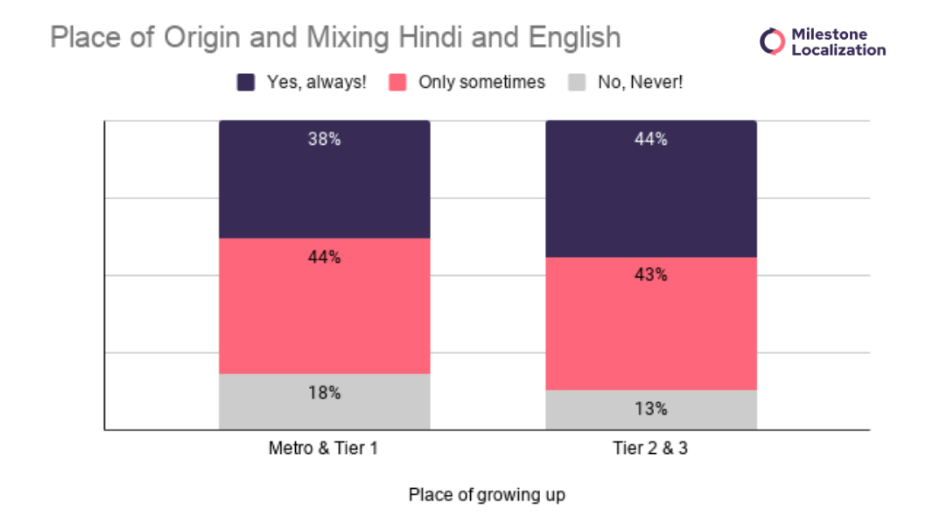
\includegraphics[width=0.8\textwidth]{plots/origin_mixing_language.png}
\end{figure}

From the above plots it can be seen that the people from the Tier 2 and 3 cities are more likely to use Hinglish than the people from the Tier 1 cities. This can be due to the more English speaking environment in the Metro cities and hence prefer to communicate in pure language instead of mixing Hindi and English.

\subsubsection{Speed of Reading}

\begin{figure}[H]
    \centering
    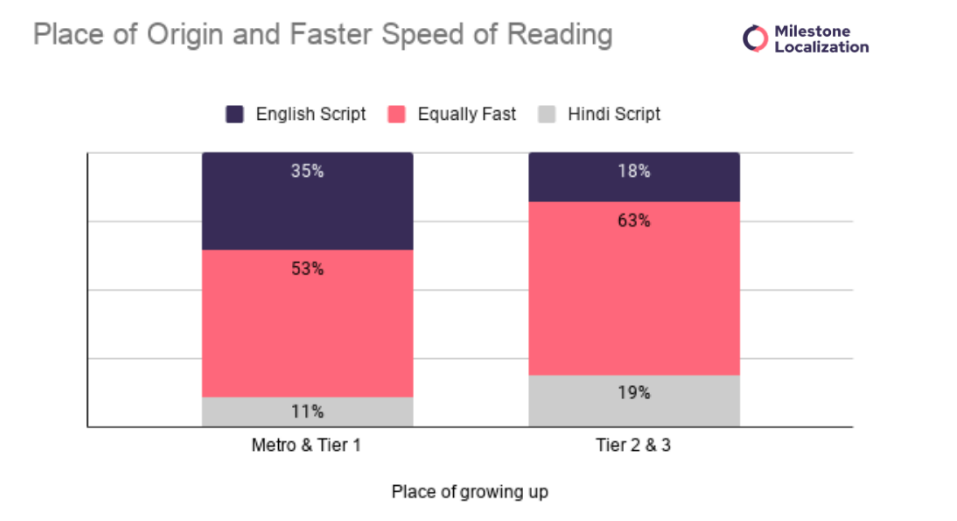
\includegraphics[width=0.8\textwidth]{plots/origin_faster_read.png}
\end{figure}

Again due to the more english speaking environment in the metro cities, the people are more comfortable in reading the English Script rather than reading the Devnagari script. Whereas in the Tier 2 and 3 cities, due to the English speaking environment not being encouraged to much extent and education still provided in both Hindi and English, the people are more comfortable in reading both Hindi and English. People in Metro and Tier 1 cities lack the speed of reading the hindi script significantly.

\subsection{Impact of Mother Tongue}

About 41.7\% percent of the people from the survey have the mother tongue as Hindi. The rest of the people are from the other mother languages. Mother Tongue can have a significant impact on the language usage and the speed of reading and other aspects of the language and we shall study them now:

\subsubsection{Mixing of Languages}

\begin{figure}[H]
    \centering
    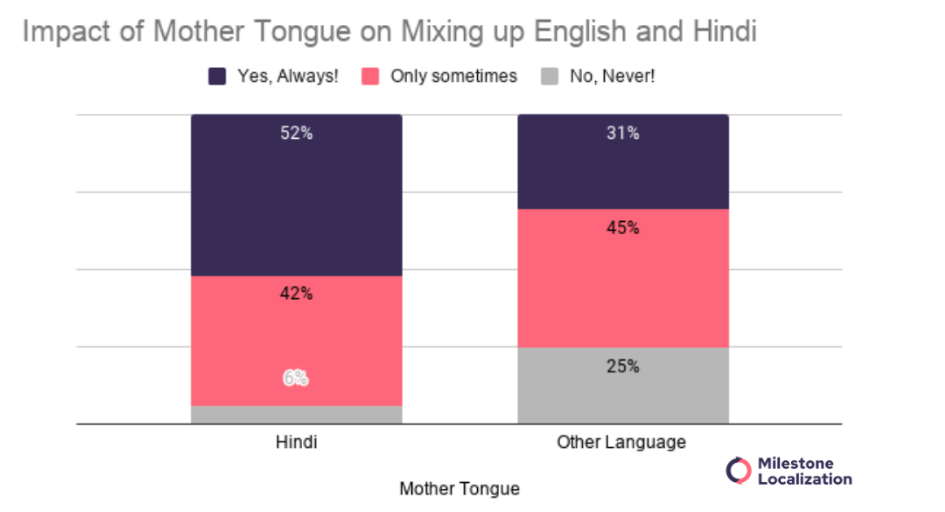
\includegraphics[width=0.8\textwidth]{plots/mother_mixing_language.png}
\end{figure}
Poeple who have Hindi as their mother tongue are more likely to use Hinglish than the people who have other mother languages. People who have Hindi as their mother languages don't use English as their medium of communication, whereas the poeple who don't have Hindi as their mother tongue are much likely to use English in it's pure form. 

\subsubsection{Speed of Reading}

\begin{figure}[H]
    \centering
    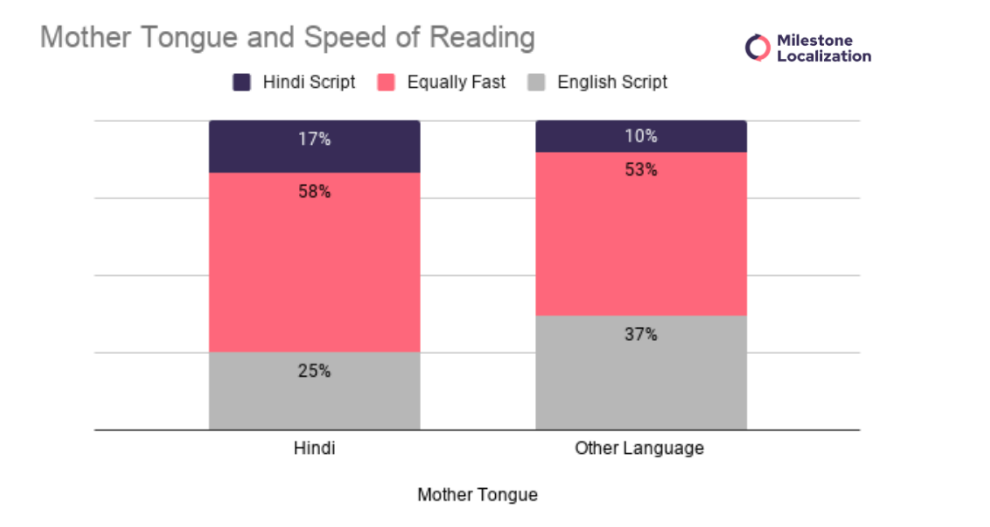
\includegraphics[width=0.8\textwidth]{plots/mother_faster_read.png}
\end{figure}
People who don't have Hindi as their mother tongue are not able to read even the Hindi words written in the English Script with pace and smoothly and prefer to read it in the English Script. So is also kind of the case with the people who have Hindi as their mother tongue, even not a large numbr of them are fluent in reading the hindi script. This is spefically happening because most of the communication and education is done in the mode of English and even thought their Mother tongue might be Hindi, it maybe just a another subject in their school curicullum.

\subsection{Frequent Usage}
36.7\% of the total responders of the survey said that they use Hindi in their day to day life more than English. While the rest of them use English in their day to day life more than Hindi. Now we will study the effect of this on various aspects of Hinglish usage.

\subsubsection{Mixing of Languages}

\begin{figure}[H]
    \centering
    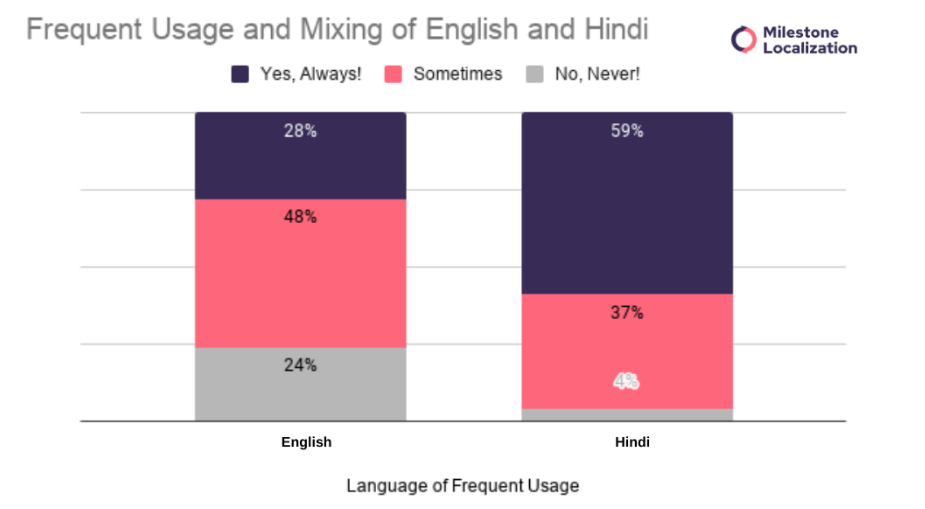
\includegraphics[width=0.8\textwidth]{plots/frequent_mixing_language.png}
\end{figure}

It can be seen that the people who use Hindi frequently use Hinglish more than the people who use English frequently. Very few of the people who use English more frequently use Hinglish. Rarely anyone is using Hindi speaks it in the pure form all the time. 

\subsubsection{Speed of Reading}

\begin{figure}[H]
    \centering
    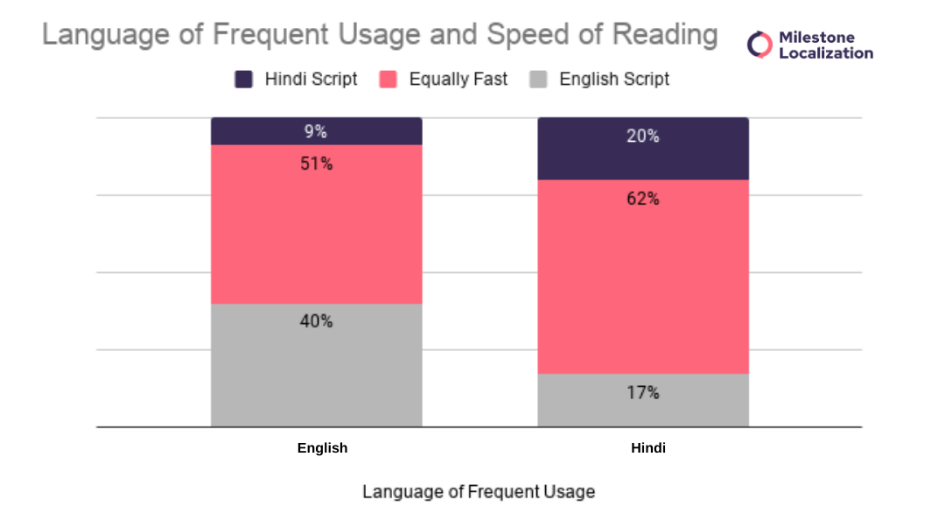
\includegraphics[width=0.8\textwidth]{plots/frequent_faster_read.png}
\end{figure}

For the people who don't use Hindi as their mother tongue, very few people are able to read the Devnagari script and most of them prefer only the English Script. This is true for the poeple who use Hindi more frequently, even they are not fluent in reading it in the pure form.

\section{Impact on Hindi and English}


\section{Conclusions}

\section{Notes and References}

\end{document}